\documentclass[10pt,twocolumn]{article}

\usepackage[a4paper,margin=1cm]{geometry}
\usepackage[utf8]{inputenc}
\usepackage[T1]{fontenc}
\usepackage[brazil]{babel}
\usepackage{amsmath}
\usepackage{listings}
\usepackage{xcolor}
\usepackage{booktabs}
\usepackage{graphicx}
\usepackage{titlesec}

% Titulos menores (orientacao recebida em aula)
\titleformat{\section}{\small\bfseries}{\thesection.}{0.4em}{}
\titlespacing*{\section}{0pt}{3pt}{1pt}
\setlength{\parskip}{0pt}
\setlength{\columnsep}{8pt}
\linespread{0.92}\selectfont

\lstset{
    basicstyle=\ttfamily\scriptsize,
    breaklines=true,
    numbers=left,
    numberstyle=\tiny,
    frame=single,
    language=C,
    keywordstyle=\color{blue},
    commentstyle=\color{gray}
}

% Gerado por benchmark/analise.py -- nao editar a mao.
\newcommand{\Tseq}{993,4}
\newcommand{\TabRef}{%
\begin{tabular}{@{}lcc@{}}
\toprule
Referência (1 core) & Tempo (s) & DP \\
\midrule
Bubble sort, vetor inteiro & 993,4 & 0,4 \\
D\&C sequencial, 2 pedaços & 499,4 & 0,1 \\
D\&C sequencial, 4 pedaços & 250,4 & 0,1 \\
D\&C sequencial, 8 pedaços & 125,5 & 0,0 \\
D\&C sequencial, 16 pedaços & 62,3 & 0,0 \\
\bottomrule
\end{tabular}}
\newcommand{\TabSem}{%
\begin{tabular}{@{}cccccccc@{}}
\toprule
p & Pedaços & Tempo (s) & DP & S & E (\%) & S$_{dc}$ & E$_{dc}$ (\%) \\
\midrule
3 & 2 & 249,49 & 0,06 & 4,0 & 133 & 2,0 & 67 \\
7 & 4 & 64,22 & 0,27 & 15,5 & 221 & 3,9 & 56 \\
15 & 8 & 16,58 & 0,06 & 59,9 & 399 & 7,6 & 50 \\
31 & 16 & 6,67 & 0,07 & 149,0 & 481 & 9,3 & 30 \\
\bottomrule
\end{tabular}}
\newcommand{\TabArtigo}{%
\begin{tabular}{@{}cccccccc@{}}
\toprule
p & Pedaços & Tempo (s) & DP & S & E (\%) & S$_{dc}$ & E$_{dc}$ (\%) \\
\midrule
2 & 2 & 498,97 & 0,11 & 2,0 & 100 & 1,0 & 50 \\
3 & 2 & 249,29 & 0,07 & 4,0 & 133 & 2,0 & 67 \\
4 & 4 & 125,34 & 0,17 & 7,9 & 198 & 2,0 & 50 \\
7 & 4 & 62,69 & 0,18 & 15,8 & 226 & 4,0 & 57 \\
8 & 8 & 31,71 & 0,20 & 31,3 & 392 & 4,0 & 49 \\
15 & 8 & 16,41 & 0,01 & 60,5 & 404 & 7,6 & 51 \\
16 & 16 & 8,24 & 0,02 & 120,6 & 754 & 7,6 & 47 \\
31 & 16 & 5,01 & 0,03 & 198,1 & 639 & 12,4 & 40 \\
32 & 32 & 3,37 & 0,01 & 294,9 & 922 & 9,2 & 29 \\
\bottomrule
\end{tabular}}
\newcommand{\TabBloq}{%
\begin{tabular}{@{}cccccccc@{}}
\toprule
p & Pedaços & Tempo (s) & DP & S & E (\%) & S$_{dc}$ & E$_{dc}$ (\%) \\
\midrule
2 & 2 & 249,87 & 0,12 & 4,0 & 199 & 2,0 & 100 \\
3 & 2 & 249,42 & 0,12 & 4,0 & 133 & 2,0 & 67 \\
4 & 4 & 62,68 & 0,09 & 15,8 & 396 & 4,0 & 100 \\
7 & 4 & 63,79 & 1,62 & 15,6 & 222 & 3,9 & 56 \\
8 & 8 & 16,08 & 0,07 & 61,8 & 772 & 7,8 & 98 \\
15 & 8 & 16,44 & 0,02 & 60,4 & 403 & 7,6 & 51 \\
16 & 16 & 4,14 & 0,02 & 240,0 & 1500 & 15,1 & 94 \\
31 & 16 & 4,77 & 0,00 & 208,1 & 671 & 13,1 & 42 \\
32 & 32 & 1,69 & 0,00 & 587,8 & 1837 & 18,4 & 57 \\
\bottomrule
\end{tabular}}
\newcommand{\TabMuitos}{%
\begin{tabular}{@{}c|cc|cc|cc@{}}
\toprule
 & \multicolumn{2}{c|}{sem balanc.} & \multicolumn{2}{c|}{artigo (Isend)} & \multicolumn{2}{c}{artigo (bloq.)} \\
p & Tempo (s) & DP & Tempo (s) & DP & Tempo (s) & DP \\
\midrule
63 & 3,553 & 0,110 & 1,968 & 0,147 & 1,953 & 0,201 \\
127 & 2,062 & 0,057 & 1,240 & 0,010 & 1,012 & 0,059 \\
255 & 1,296 & 0,042 & 0,704 & 0,036 & 0,813 & 0,326 \\
511 & 2,296 & 0,358 & 1,503 & 0,507 & 1,351 & 0,265 \\
1023 & 3,380 & 0,136 & 2,117 & 0,185 & 2,385 & 0,169 \\
\bottomrule
\end{tabular}}
\newcommand{\TabCiclico}{%
\begin{tabular}{@{}lccc@{}}
\toprule
Versão & p & Em bloco (s) & Cíclica (s) \\
\midrule
sem balanceamento & 15 & 16,58 & 16,48 \\
sem balanceamento & 31 & 6,67 & 6,62 \\
artigo, envio bloqueante & 16 & 4,14 & 4,13 \\
artigo, envio bloqueante & 31 & 4,77 & 4,80 \\
artigo, envio bloqueante & 32 & 1,69 & 1,69 \\
\bottomrule
\end{tabular}}


% Procura os fontes na propria pasta do main.tex, em src/ ou em ../src/.
\newcommand{\includecodigo}[1]{%
  \IfFileExists{#1}{%
    \lstinputlisting[language=C]{#1}%
  }{%
    \IfFileExists{src/#1}{%
      \lstinputlisting[language=C]{src/#1}%
    }{%
      \IfFileExists{../src/#1}{%
        \lstinputlisting[language=C]{../src/#1}%
      }{%
        \textbf{Arquivo \texttt{#1} não encontrado.}%
      }%
    }%
  }%
}

\title{\vspace{-1.5cm}\large Bubble sort por divisão e conquista com MPI:
sem balanceamento e com o balanceamento do artigo\vspace{-0.3cm}}
\author{
    \normalsize
    Bruno Neves \quad
    Guilherme Hoffmann \quad
    João Sbardelotto \\
    \small Computação Paralela --- Turma 320 --- Prof. Cesar A. F. De Rose ---
    PUCRS --- Grupo 12
}
\date{\vspace{-0.6cm}}

\begin{document}
\maketitle
\thispagestyle{empty}

\section{Problema e unidade de trabalho}

Ordenamos 1.000.000 de inteiros em ordem decrescente, o pior caso do bubble sort,
com a rotina do enunciado; geração e conferência ficam fora da medição. A
divisão e conquista forma uma árvore binária: a raiz gera o vetor, divide-o ao
meio, cada filho repete a decisão e as folhas ordenam com bubble sort; o pai
intercala as metades ordenadas e devolve o resultado. O eixo paralelizado é a
posição no vetor; a unidade é um subvetor contíguo.

Como o bubble sort é $O(n^2)$, dividir o vetor em $L$ pedaços reduz o trabalho
total por $L$: a referência sequencial com $L$ pedaços leva aproximadamente
$T_s/L$ --- 499,4, 250,4, 125,5 e 62,3~s para $L=2,4,8,16$. Esse ganho
algorítmico não é paralelismo e precisa ser separado dele.

\section{Modelo de divisão e conquista e diretivas MPI}

O programa é SPMD. Os processos formam a árvore da Figura~1, com filhos $2r+1$
e $2r+2$ e pai $(r-1)/2$. A raiz inicializa o vetor; cada outro processo recebe
do pai com \texttt{MPI\_Probe} e \texttt{MPI\_Get\_count}, que dão o tamanho da
mensagem, e \texttt{MPI\_Recv}. Se o pedaço é maior que \texttt{delta} e o filho
da direita existe, o processo divide: envia uma metade a cada filho com
\texttt{MPI\_Send}, espera as duas metades com \texttt{MPI\_Recv} e as
intercala. Senão, conquista com bubble sort. O resultado volta ao pai com
\texttt{MPI\_Send}; a intercalação é feita pelo pai, que conhece as duas metades.

Na versão sem balanceamento, \texttt{delta} = $\lceil n/\text{folhas}\rceil$, em
que folhas é o número de folhas da maior árvore cheia que cabe em $p$
processos. Quem não recebe trabalho não fica preso no \texttt{MPI\_Recv}.
Só as folhas ordenam; os nós
internos passam a execução esperando os filhos e só trabalham na intercalação.

A versão com balanceamento é a do artigo de Radenski. O processo não entrega as
duas metades: no nível $L$, envia a segunda metade ao ajudante $r+2^L$ com
\texttt{MPI\_Isend} e continua ordenando a primeira, descendo um nível. Depois
recebe a segunda metade, intercala e devolve ao pai. A condição de parada não tem
\texttt{delta}: se o ajudante não existe ($r+2^L >$ último rank), o processo
ordena sozinho. A profundidade sai de $p$: com $p=2^k$ todos ordenam $n/p$; com
$p=2^k-1$ um processo fica com o dobro.

Trocamos o \texttt{MPI\_Isend} por \texttt{MPI\_Send} (versão bloqueante): a
mensagem é grande e o pai não volta ao MPI durante o bubble sort, então o
ajudante só recebia depois, serializando os trabalhos. Com o envio bloqueante,
o ajudante, já em \texttt{MPI\_Probe}, começa junto. Os tempos por atividade
são reunidos na raiz por \texttt{MPI\_Gather} fora da medição.

\section{Ambiente e metodologia}

Dois nós exclusivos da atlântica (LAD), cada um com 2 Xeon E5520, 8 núcleos
físicos e 16 CPUs lógicas (HT), ligados por Ethernet Gigabit. Open MPI 4.1.1,
\texttt{srun -N 2 -n $p$}. Vetor de 1.000.000 de inteiros, 5 execuções por ponto,
e $T_s = \Tseq \pm 0{,}4$~s. A referência D\&C sequencial usa a mesma árvore e
\texttt{delta} em 1 core. Foram medidas 1, 3, 7, 15 e 31 processos; a versão do
artigo também com 2, 4, 8, 16 e 32; e 63, 127, 255, 511 e 1023 com
\texttt{--overcommit}. A distribuição dos ranks foi a padrão em bloco e, em
testes, a cíclica (\texttt{-m cyclic}). Todas as execuções terminaram ordenadas.

Dois speed-ups são reportados. $S = T_s/T_p$ é o do enunciado, mas é superlinear
porque a divisão reduz o trabalho total. $S_{dc} = T_{dc}(L)/T_p$ compara com a
mesma divisão em 1 core, e $E_{dc} = S_{dc}/p$ mostra quantos dos $p$ processos
estão de fato ordenando. $E_{dc}=100\%$ significa que todos ordenaram pedaços
iguais, sem perda; $E_{dc}=50\%$ é o teto da versão sem balanceamento.

\section{Análise dos resultados}

\textbf{Ganho algorítmico e as duas eficiências.} O $S$ do enunciado chega a
294,9$\times$ com 32 processos na versão do artigo e a 587,8$\times$ na versão
bloqueante, com $E$ de 922\% e 1837\%. Isso vem de dividir um problema
$O(n^2)$; a leitura correta é $S_{dc}$ e $E_{dc}$. Na versão bloqueante, $E_{dc}$
é 100\% com 2 e 4 processos, 98\% com 8, 94\% com 16 e 57\% com 32. Até 8
processos o ganho do paralelismo é quase integral; em 16 e 32 entram a
comunicação e o HT.

\textbf{Sem balanceamento.} Só as folhas ordenam, e com $p=2^k-1$ há $(p+1)/2$
folhas. O teto de $E_{dc}$ é cerca de 50\%, e o medido cai de 67\% ($p=3$) para
56\% ($p=7$), 50\% ($p=15$) e 30\% ($p=31$). Em $p=15$, o nível 3 ordena
16,4~s e os níveis 0 a 2 esperam o mesmo tempo. Em $p=31$, os 16 processos do último nível
dividem 8 núcleos físicos via HT e ordenam 62.500 elementos em 6,5~s, não em
3,9~s; o tempo total, 6,67~s, é 2,5$\times$ menor que o de $p=15$, e não
4$\times$, porque o HT não acrescenta capacidade de cálculo.

\textbf{Artigo: \texttt{MPI\_Isend} e envio bloqueante.} Com \texttt{Isend}, o
tempo dobra nas potências de dois: 499,0 contra 249,9~s com $p=2$; 125,3 contra
62,7~s com 4; 31,7 contra 16,1~s com 8; 8,24 contra 4,14~s com 16; 3,37 contra
1,69~s com 32. O ajudante só recebe depois que o pai termina seu bubble sort;
com \texttt{MPI\_Send} ele começa junto. Nas contagens 3, 7 e 15 Isend e
bloqueante empatam (249,3/249,4; 62,7/63,8; 16,41/16,44~s).

\textbf{Condição de parada e potências de dois.} Com $p=2^k$ o artigo divide o
vetor em $p$ pedaços iguais; com $p=2^k-1$ a árvore fica torta e um processo
recebe o dobro. É por isso que $p=15$ leva 16,44~s e $p=16$ leva 4,14~s
(4$\times$), e $p=31$ leva 4,77~s contra 1,69~s de $p=32$. Nessas contagens ela
empata com a sem balanceamento ($p=3$: 249,4/249,5; $p=7$: 63,8/64,2; $p=15$:
16,44/16,58~s); o balanceamento pleno só aparece com $p$ potência de dois. A
distribuição cíclica não muda o resultado (diferenças abaixo de 0,1~s), porque o
gargalo é o processo sobrecarregado, não o nó.

\textbf{Muitos processos e HT.} O melhor tempo fica em 255 processos: 0,704~s
com \texttt{Isend}, 0,813~s com envio bloqueante e 1,296~s sem balanceamento.
Acima disso o tempo sobe --- com 1023 processos, 2,117, 2,385 e 3,380~s. Acima de
32 há \emph{overcommit} nas 32 CPUs lógicas e o custo de lançamento e
comunicação domina. Em 32 processos o HT explica a queda de $E_{dc}$ de 94\%
para 57\%: 32 processos em 16 núcleos físicos deixam cada bubble sort cerca de
1,7$\times$ mais lento.

\section{Uso de ferramentas de IA}

Foi usado o Claude (Anthropic), pelo Claude Code, com revisão do grupo, na
leitura do enunciado, no artigo e código do Radenski, no C/MPI, nos scripts de
medição e análise, na execução no LAD, nas tabelas/gráficos e na redação.

\section{Conclusão}

A versão bloqueante chegou a 240,0$\times$ ($S$) e 15,1$\times$ ($S_{dc}$) com 16
processos, e a 587,8$\times$ e 18,4$\times$ com 32; a sem balanceamento para em
149,0$\times$ e 9,3$\times$ com 31. O limite é o processo que recebe o dobro
quando $p$ não é potência de dois e o HT acima de 16 processos. O ganho
algorítmico da divisão (fator $L$) supera o de paralelismo; $S$ não é speed-up
paralelo. A versão do artigo só balanceia de fato com $p$
potência de dois; com $p=2^k-1$ empata com a sem balanceamento. Para mensagens
grandes e sem progresso, o \texttt{MPI\_Isend} não ajuda, e o envio bloqueante é
melhor.

% =====================================================
% PAGINA 2 --- TABELAS E GRAFICOS (coluna simples)
% =====================================================
\clearpage
\onecolumn
\section*{Tabelas e gráficos}
\vspace{-4pt}
\noindent\small Dois nós da atlântica (2$\times$ Xeon E5520 por nó, 8 núcleos
/ 16 CPUs lógicas, Ethernet Gigabit). Vetor de 1.000.000 de inteiros em ordem
decrescente, 5 execuções por ponto. $T_s = \Tseq \pm 0{,}4$~s; $p$ = processos
MPI. $S = T_s/T_p$ e $E = S/p$; $S_{dc} = T_{dc}(L)/T_p$ e $E_{dc} =
S_{dc}/p$, com $T_{dc}(L)$ a D\&C sequencial de $L$ pedaços (499,4, 250,4,
125,5 e 62,3~s para $L=2,4,8,16$).

\vspace{2pt}
\noindent
\begin{minipage}[t]{0.49\linewidth}
\centering\small
\textbf{Sem balanceamento}\\[2pt]
\scriptsize\TabSem
\end{minipage}
\hfill
\begin{minipage}[t]{0.49\linewidth}
\centering\small
\textbf{Artigo (\texttt{MPI\_Isend})}\\[2pt]
\scriptsize\TabArtigo
\end{minipage}

\vspace{2pt}
\noindent
\begin{minipage}[t]{0.49\linewidth}
\centering\small
\textbf{Artigo (envio bloqueante)}\\[2pt]
\scriptsize\TabBloq
\end{minipage}
\hfill
\begin{minipage}[t]{0.49\linewidth}
\centering\small
\textbf{Distribuição em bloco $\times$ cíclica}\\[2pt]
\scriptsize\TabCiclico
\end{minipage}

\vspace{2pt}
\begin{center}
\small\textbf{Mais processos que CPUs}\\[2pt]
\scriptsize\TabMuitos
\end{center}

\vspace{4pt}
\begin{center}
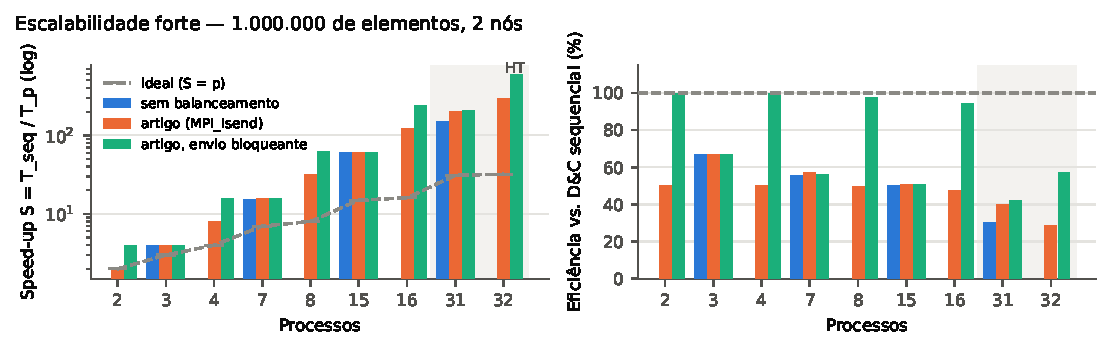
\includegraphics[width=0.66\linewidth]{fig_forte.pdf}\\[1pt]
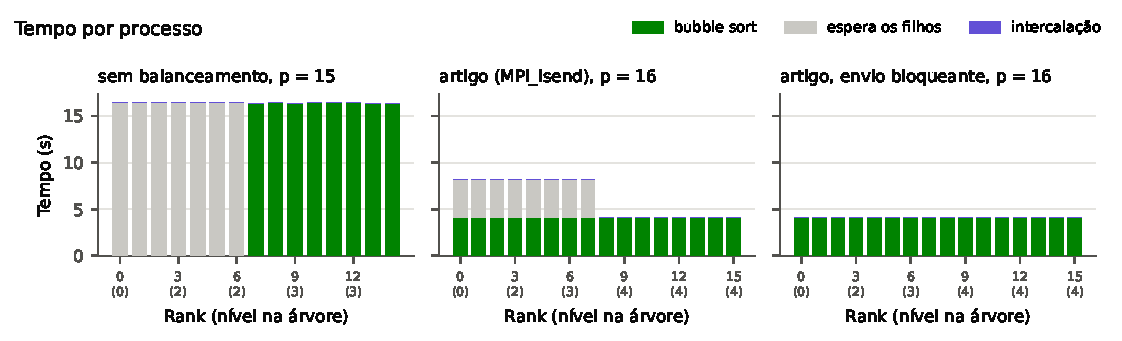
\includegraphics[width=0.66\linewidth]{fig_niveis.pdf}\\[1pt]
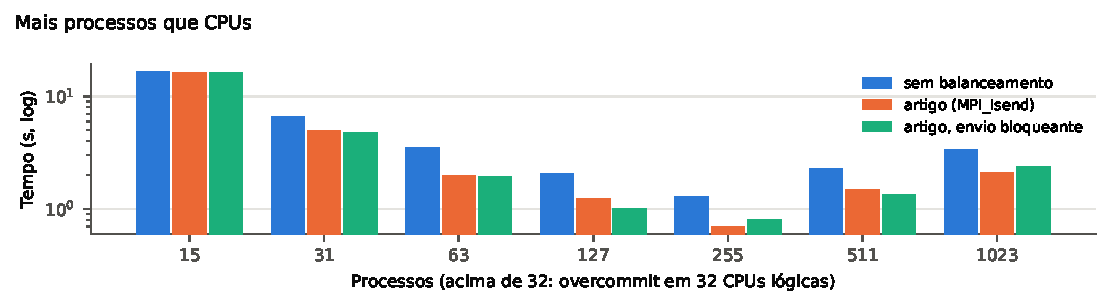
\includegraphics[width=0.66\linewidth]{fig_muitos.pdf}
\end{center}

% =====================================================
% PAGINA 3+ --- CODIGO-FONTE (coluna simples, sem limite)
% =====================================================
\clearpage
\section*{Código-fonte --- versão sem balanceamento (MPI)}
\includecodigo{dc_mpi.c}

\clearpage
\section*{Código-fonte --- versão do artigo, com balanceamento (MPI)}
\includecodigo{dc_artigo_mpi.c}

\clearpage
\section*{Código-fonte --- bubble sort sequencial e D\&C de referência}
\includecodigo{bs_seq.c}

\end{document}
